\chapter{TCP}
\label{chap:tcp}




Wireshark抓包HTTPS

\begin{lstlisting}[style=cshell]
mkdir ~/tls && touch ~/tls/sslkeylog.log

#zsh
echo "\nexport SSLKEYLOGFILE=~/tls/sslkeylog.log" >> ~/.zshrc && source ~/.zshrc

# bash
echo "\nexport SSLKEYLOGFILE=~/tls/sslkeylog.log" >> ~/.bash_profile && . ~/.bash_profile

# 启动
./Google\ Chrome --ssl-key-log-file=~/tls/sslkeylog.log
\end{lstlisting}


\begin{figure}[H]
        \centering
        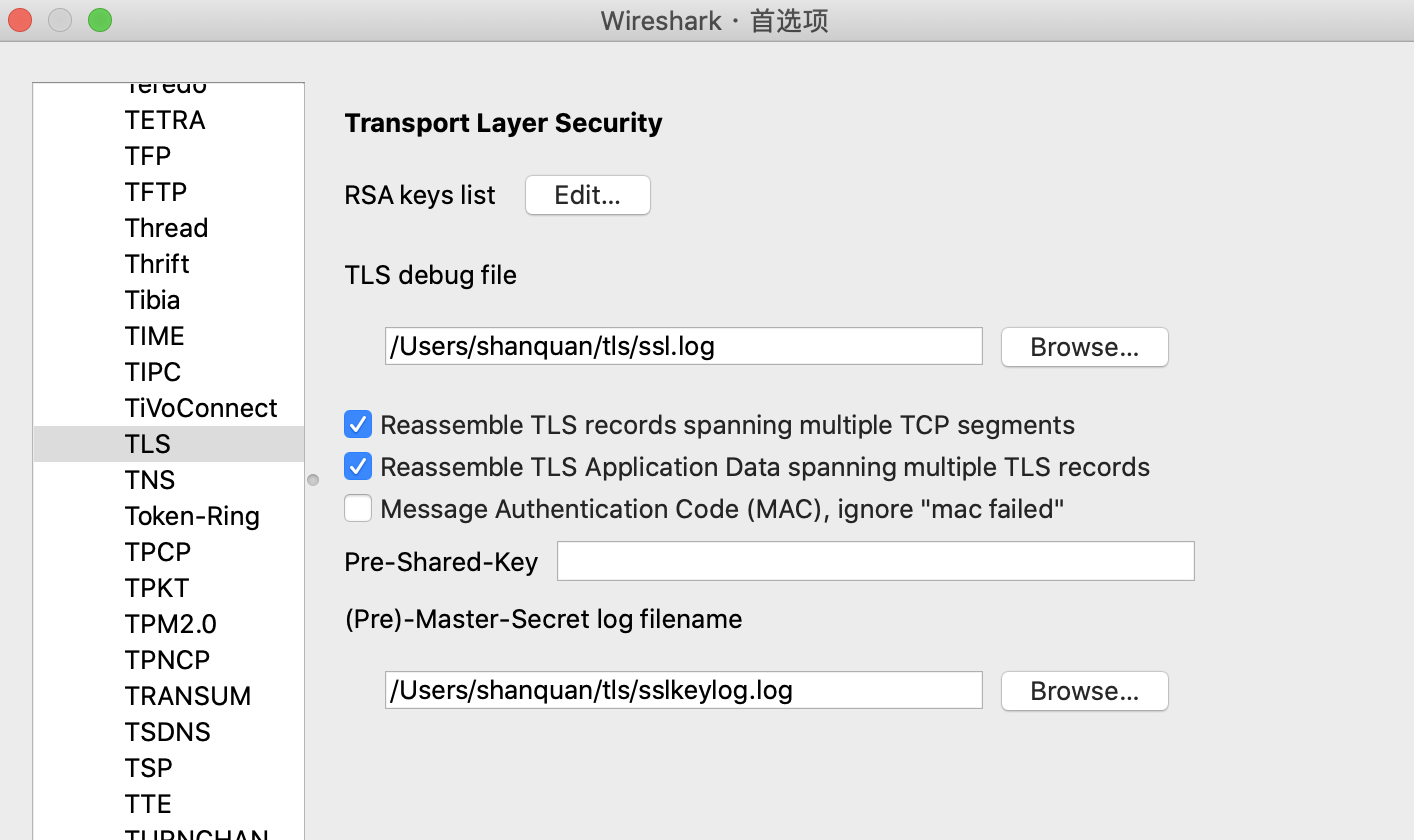
\includegraphics[width=1\textwidth]{tcp/tcp_https_ sslkeylog.jpg}
        \caption{HTTP 时间轴}
    \end{figure}


    
\href{https://developer.mozilla.org/en-US/docs/Mozilla/Projects/NSS/Key_Log_Format}{NSS}